\section{Introduction}
\label{sec:intro}

\paragraph{Motivation}
Programming applications that interact with physical processes are becoming central in  robotics, manufacturing, IoT, and other cyberphysical systems (CPS).  Following the trends in the cloud and smartphone ecosystems, programmability is going to become  important in these domains as platform become more open and hardware developers shift to the  applications marketplace. Unfortunately, {\em domain specific languages (DSL)\/} for these domains are surgically platform dependent, and they combine  low-level sensing, communication, and control tasks with the application-level logic~\cite{nordmann2014robotics}. This  tight-coupling of applications with platform-specific details can hinder development, modularity, portability, code reuse, and testing. 

This need for raising the level of abstraction and separating the \emph{platform-independent} from the \emph{platform-dependent} concerns motivates our work in this paper. Consider for a moment, the task of developing an application for distributed package delivery with mobile robots in a building. The higher-level coordination has to deal with assigning robots to visit way-points in different rooms, load-balancing, and mainteinence schedules.  For all of the reasons mentioned above, these coordination tasks {\em should be\/} separated from the  steering control of the individual vehicles, indoor positioning, and message-level communication protocols tied to the specific hardware platforms. 

Current programming languages do not natively support such separation of concerns. They do not have the high-level abstractions needed for programming distributed cyberphysical systems.  The developer will have to keep track of communication between different sensors, actuators, and program variables. The {\em robotic operating system (ROS)}~\cite{rosbridge_suite,ros} does provide useful libraries and  publish-subscribe messaging standards, but these are not integrated in a programming abstraction. Similarly, coordination across multiple robots has to be built from the ground up using message passing threads. In order to simulate and test the application, one has to create different threads or instances for the developed code corresponding to different agents, and on top of that, the agent programs have to be harnessed in a physical world simulator with proper sensor and actuator models. In order to analyze correctness, one has to first define the semantics of the system---a difficult proposition in an of itself, given the concurrency and data flows in multiple time-scales. 

%A further source of concern is the gap between the system model with iand the executable code that is actually . 

Our project aims to address some of these challenges by designing, developing, and evaluating an open source programming system for distributed robotics. \footnote{Links and references to the project as well as downloadable software will be made available to the PC chairs. We omit the information here for the sake of maintaining anonymity.} In this paper, we present for the first time the design and the implementation of the  {\em $\lgname$ language} and the supporting software tools, namely the compiler, the \K executable semantics, and the simulator. These components form the  core of the programming system. $\lgname$ programs have been deployed on F1/10 vehicles, quadcopter, and roombas, and the results related to hardware deployment will be presented in a future article. 





%
%\begin{figure}[h!]
%\centering
%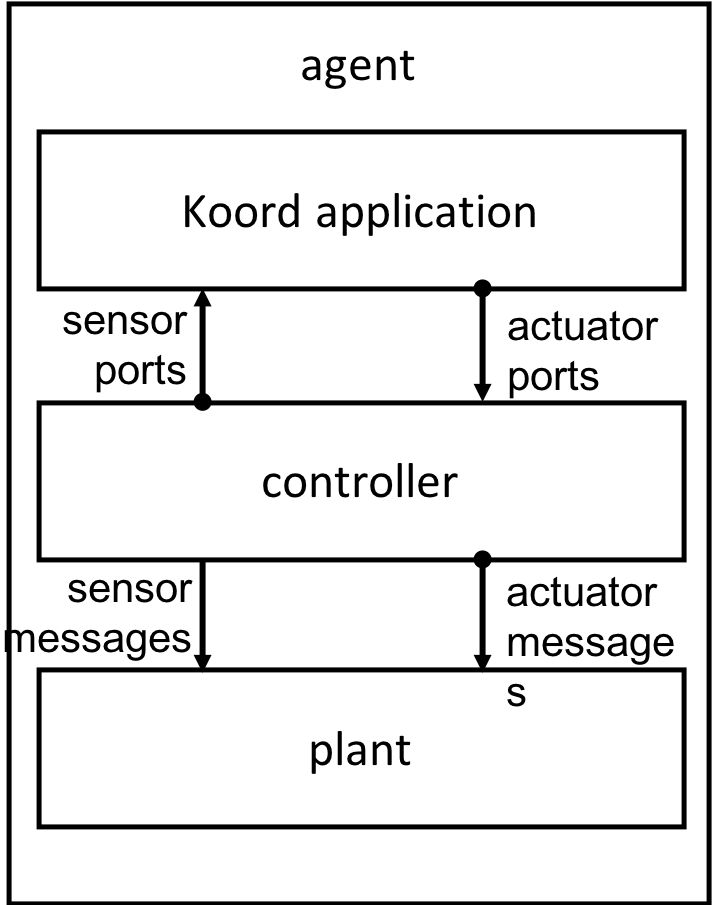
\includegraphics[width=0.48\textwidth]{figs/arch.png}
%\caption{\small CyPhyHouse framework. Major tools shown in blue.}
%\label{fig:arch}
%\end{figure}
%
\subsection{Contributions of the paper}
\subsubsection{Design and implementation of $\lgname$ language}
{\em We present a clean-slate design and implementation of an event-triggered programming language, for distributed cyberphysical systems, namely $\lgname$.} 
%
$\lgname$ combines distributed shared memory abstraction for coordination across agents and a synchronous model of communication with the physical environment through sensors and actuators. Individual agent programs, which may be concurrent, are written in a familiar precondition-effect style language.
%

Consider a simple line-formation program in which a set of $\NMAX$ robots form a equi-spaced line starting from arbitrary positions. The textbook algorithm is for each robot $i$ to repeatedly move towards the midpoint of the line joining the positions of $i-1$ and $i+1$. The extremal robots with ids $0$ and $\NMAX -1$ stay fixed. This is a archetypal protocol for synchronization, pattern formation, and consensus~\cite{Tsitsiklis:1986,Blondel,Magnusbook2010,Fax} in distributed robotics.
%
% \belowcaptionskip=-10pt
\begin{figure}
\begin{mdframed}
\label{fig:lineform}
        {\lstinputlisting[language=koordnums,frame=None]{code/lineform.tex}}
\end{mdframed}
\caption{Lineform $\lgname$ program}

\end{figure}
The above $10$ line  $\lgname$ program implements this line formation algorithm and can be simulated or deployed (see Figure~\ref{fig:shapeplots}). Among these $10$ lines of code, lines 1-5 import the {\em controller module\/} called {\em Motion\/} that enables this program to access the sensor port with the agent's position $(\mathit{psn})$ and the actuator port $(\mathit{target})$. An implementation of  a {\em controller module\/} has platform-specific path planners and low-level controllers for moving specific types of robots in the physical world. {\em Thus, with different implementations of the {\em Motion\/} interface the $\mathit{Lineform}$ $\lgname$  program can be ported to different platforms\/}. 

Another powerful feature of $\lgname$ used in the $\mathit{Lineform}$ program is the single-write multi-reader ({\bf allread}) shared array $x$, in which component $x[i]$ records the position of the $i^{th}$ robot in each round.  Shared variables allow the participating agents programs to coordinate without exposing the programmer to explicit message passing channels, buffers, and threads. This makes $\lgname$ programs succinct, readable, and often, as in the  above example, remarkably close to the textbook version of the algorithm. The $\lgname$ runtime system (discussed in more detail in Section~\ref{sec:software}) implements the propagation of  the shared variable write over messages. The formalization of the resulting semantics is discussed in Section~\ref{sec:semantics}.

%
The one and only event in the $\mathit{Lineform}$ program is $\mathit{TargetUpdate}$ (lines 5-9): it updates the target position of the agent  to be the midpoint of its neighbors.  Figure~\ref{fig:shapeplots} shows the result of simulating a slightly modified version of $\mathit{Lineform}$ on the $\lgname$ simulator with $25$ robots forming a 3D-shape. The $\lgname$ compiler can also generate executables that can be deployed on several mobile robotic hardware platforms such as F1/10 cars~\cite{f110}, drones, and Roombas. 
%\renewcommand{\lstinputlisting}[1][]{\oldlstinputlisting[frame=lines,#1]}
 
%\begin{figure}[ht!]
%	\label{fig:lineform}
%	\noindent
%	\begin{center}
%		\scriptsize
%		\two{0.4}{0.6}
%		{\lstinputlisting[language=xyzNums,frame=lines]{code/lineform.tex}}
%	\par        
%	\end{center}
%	\caption{\small $\lgname$ program for line formation ({\em Left}) and its mathematical counterpart in robotics and control textbooks ({\em Right}).}
%\end{figure}

%The shared \emph{allread} variable $p$ (Line\ref{lineformp}) is used by the agents to communicate their position to the other robots. The function \emph{midpoint} is a part of the library functions provided for the data type \emph{pos}; where $$\mathit{midpoint}(p_1,p_2,\ldots,p_n) = pos(\frac{\Sigma_n p_i.x}{n},\frac{\Sigma_n p_i.y}{n},\frac{\Sigma_n p_i.z}{n}) $$.
%

%We have implemented a compiler for $\lgname$ that generates executable Python programs that can be either simulated in a discrete event simulator (discussed below) or 

\subsubsection{First formalization of a robotics or CPS language in \K}
% motivation
Implementations of programming languages usually contain many bugs. One common type of bugs creeps in from the gap between the official semantics of the language (as in a user manual) and the its implementation as embodied in a compiler. The \K framework~\cite{rosu-serbanuta-2013-k} closes this gap by allowing the specification of {\em  formal executable semantics of any programming language} in terms of rewrite rules. These rewrite rules define how each and every possible statement in the  language changes, possibly nondeterministically, the ``state of the machine'' executing the program. 
%
\K  provided the most complete to-date formalization  of the C language~\cite{KC}. This semantics was tested against the GCC torture test suite and it successfully passed 99.2\% of 776 test programs. Recently, \K  was used to provide a formal semantics of x86-64~\cite{rosuadvepaper} and the Ethereum Virtual Machine (EVM) bytecode. 


%\K  using computations over states or configurations, and rewrite rules for said configurations. \K has several additional features including non deterministic execution, underspecification and explicit read-only and write only specifications for rewrite rules which makes \K suitable for defining concurrent and control intensive languages. 
{\em In order to close the above-mentioned gap, we have developed the complete executable formal semantics of $\lgname$ in \K.} This is the first formalization of a robotics or a CPS or a multi-agent language in \K. One  technical challenge here is to define the ``state of the machine'' executing $\lgname$ programs. This state now has to include not only the states of the program variables of the different agents, but also the sensor and actuator ports reflecting the state of the physical world, and the state of shared variables as implemented over messages.

%\sayan{
Our key innovation for achieving this formalization is to parameterize the semantics with a set of {\em environment functions\/} that model the behavior of the physical environment, the controller, and other operations that are external to the application program.  The environment functions are called by the  back-end of \K to update certain state components (e.g., sensor and actuator ports). Thus, the formal semantics of $\lgname$ is also modular and portable across  different environment models. 
%}

%ontroller behaviors with path-planners to the back-end of \K to specify rewrite rules for them, as the $\lgname$ language itself lets the user use predefined controller modules.

$\lgname$ programs have a discrete event loop, which executes periodically to interact with the environment. We can view the semantics of  $\lgname$ as a nondeterministic, timed automaton~\cite{TIOAmon}: there is a {\em sampling parameter\/} $\delta > 0$; every $\delta$-time units {\em at most one event} of the agent's program executes. This execution takes zero logical time and corresponds to a transition of the timed automaton. $\lgname$ provides distributed shared variable abstraction for programming multiple agents, which can be written to during an event execution. The consistency semantics implemented here is that the writes to shared variables are propagated to all the agents, and become visible to other agents reading the variable after one round ($\delta$ time units). In the fault-free synchronous model considered here, any number of gossip-based algorithms can be used to implement this semantics in the $\lgname$ runtime system. 


Our \K implementation of $\lgname$ enables us to execute  programs \emph{semantically accurately}. One of the factors resulting in nondeterminism is the order in which agents execute their events, and we can use the \K support for nondeterminism to generate and search all possible nondeterministic behaviors in bounded executions for a given program. To further support formal analysis in case of non-specific initial states, we also implemented an interval arithmetic in \K, and support execution of $\lgname$ programs where the initial values of variables are provided in intervals. We implemented a {\em $\lgname$ bounded-model-checking (\kbmc)\/} tool on top of the \K semantics. While the state space explosion due to the nondeterminism and distributed nature of the CPS applications makes it difficult for $\kbmc$ to scale to beyond a handful of agents, the tool is useful for finding bugs in smaller instances. For instance, in a platooning application written in $\lgname$ (\refsect{platooning}), $\kbmc$ can be used to determine the value of the sampling parameters for which the safety invariant is violated.

%Design and development of the $\lgname$ programming language and the supporting $\mathbb{K}$-based~\cite{Kpaper} verification tool \kbmc\, are discussed here for the sake of completeness; those details will appear elsewhere\footnote{}.
\begin{figure}[h!]
\begin{minipage}{0.5\textwidth}
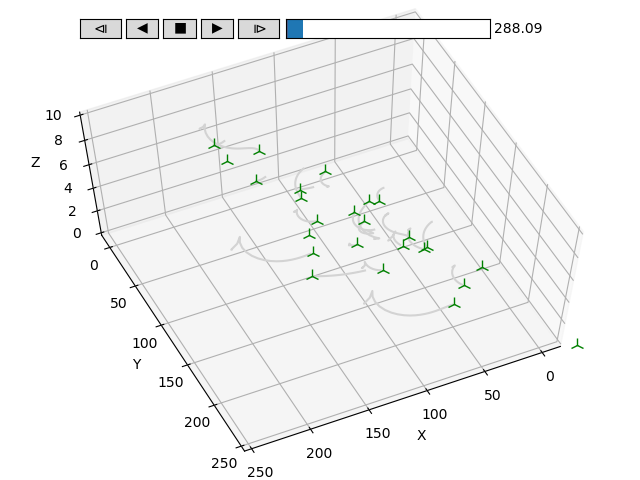
\includegraphics[width=.5\textwidth]{figs/formation1.png}\hfill
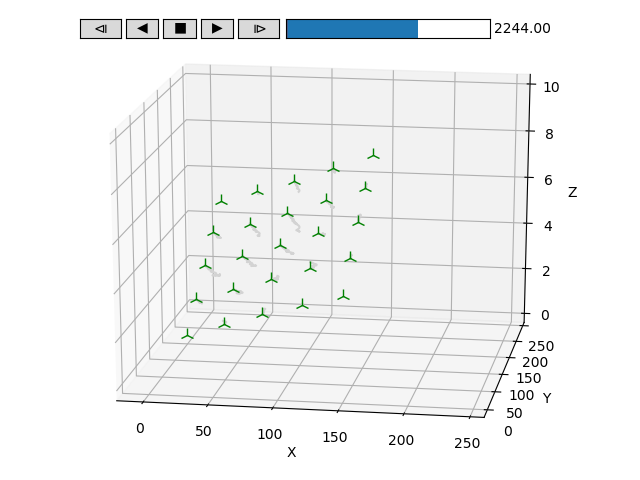
\includegraphics[width=.5\textwidth]{figs/formation4.png}\hfill%
%\includegraphics[width=.3\textwidth]{figs/Platooning_2.png}}\hfill%
\end{minipage}%
\caption{Screenshot of $\lgname$ simulator visualizing positions of a swarm of $25$ agents running a slightly modified version of $\mathit{Lineform}$ application forming a 3D-shape in space.}
\label{fig:shapeplots}
\end{figure}

\subsubsection{$\lgname$ simulator and applications}

{\em We have developed a high-fidelity, multi-threaded simulator for $\lgname$ applications.} The simulator can execute instances with 50+ agents with heterogeneous dynamics, executing $\lgname$ applications, and therefore, it is a powerful tool for debugging and performance analysis.  

The major challenges involved in designing a simulator  engine with multiple threads for each agent for managing event loops, messaging, and sensor-actuator updates. 
%\sayan{But this is on the surface an impossible task.}
The simulator uses a {\em motion automaton\/}, which can be instantiated to simulate different robot dynamics, sensors, etc. The communication protocols to propagate shared memory messages between agents are also a part of the simulator communication module. The time between two computational steps (or discrete event loop iterations) is used to propagate messages to implement shared memory as in the actual hardware stack. 
The versatile nature of the $\lgname$ and the simulator are illustrated further with three examples---platooning,  swarm formations, and distributed task allocation---in Section~\ref{sec:experims}.

The rest of the paper is organized as follows:
In Section~\ref{sec:related}, we resent a brief discussion of related research. In Section~\ref{sec:semantics}, we present the detailed semantics of $\lgname$ including the executable semantics in \K. In section \refsect{software}, we give an overview of the supporting software we have developed including the runtime system for executing $\lgname$ programs and $\kbmc$. We present the applications in \refsect{experims} and conclude in Section~\ref{sec:conclusion}.

%The simulator enables the user to test their discrete event loop with simple motion models to test and debug the application program logic without incurring the cost of hardware deployment in case of buggy programs. 
%The simulator also serves as a visualization tool as it can be used to plot the behavior of any program variables, or controller variables. For instance, we implemented a robot \emph{formation} app in $\lgname$, where several robots form a shape in which they are evenly distributed.






%\subsubsection{Other by-products}


%Design and development of the CyPhyHouse open source software system. This includes a discrete event simulator for distributed robotic systems, the application launcher, the run-time logging and monitoring system, and an integrated indoor positioning system. All of these software tools are integrated with our new robot programming language called $\lgname$ and its compiler. 





%Design and development of the Koord programming language and the supporting verification tool KoordBMC~\cite{koordreport}--- significant, related but separate efforts---are not contributions of the current paper; we discuss their usage for the sake of completeness. 
% completely describing the framework. 
% the Demonstration of an example application development using CyPhyHouse tools and deployment on a physical system using multiple quadcopters.
%Non-contributions: Spell these out  to avoid misdirected criticisms and conflict with overlapping publications.
%\begin{itemize} 
%\item Language design
%\item Verification tools.
%\item Low-level controller design for vehicles.
%\end{itemize} 

%\begin{figure}[h!]
%\centering
%\includegraphics[width=0.45\textwidth]{figs/exp_traces.png}
%\caption{\small Experimental run in our testbed. The traces show the path of each robot for the last $2$ seconds. }
%\label{fig:exp_traces}
%\end{figure}

%
%%\footnote{\href{https://cyphyhouse.github.io/index.html}{https://cyphyhouse.github.io}}: an open source software framework for programming, rapid deployment, and testing of distributed robotics applications. 
%\sayan{The high-level $\lgname$ language enables users to write succinct distributed coordination applications without getting bogged down by messaging and thread management issues (See Examples in \reffig{lineform} and \reffig{taskapp}).}
%Using the CyPhyHouse framework around $\lgname$, a user can code, compile, launch, and run applications in a highly-automated fashion (\reffig{arch}). 
%\sayan{The framework has been built over three years and has more than 100k lines of source code.}


    
    \section{Related work}
    \label{sec:related}
    Modern programming languages like C\# and Swift, and   compiler infrastructures like LLVM~\cite{llvm} have revolutionized the application development ecosystem in mobile computing.
%\paragraph*{D.} 
Inspired by these successes, there is a surge of interest in open and portable languages that raise the level of abstraction~\cite{Buzzlanguage,Bohrer:2018:VVC:3192366.3192406,reactlang,williams2003model} (For an earlier survey of Domain Specific Programming Languages (DSLs) for robotic systems see~\cite{Nordmann2014}. Most of these older languages are proprietary or generate executable files that are tied to specific platforms). 
%
Buzz~\cite{Buzzlanguage} and React~\cite{reactlang} fall in this category as does our language $\lgname$. 
The Live Robot Programming language~\cite{campusanofabry:lrp2016} not only provides a higher-level programming abstraction in terms of nested state machines, but also allows the program to be changed while running, hence reducing the feedback loop across writing, compiling, and testing of robot programs. 
%The goals of React language for robotics aligns with our goals~\cite{react-lang}
Buzz currently does not  connect with  verification tools, and the verification approach implemented with React uses precise models of the environment and performs model checking using dReal~\cite{Gao2013}. 
%Our approach is also similar in spirit to the Reactive Model-based Programming Language (RMPL)
%~\cite{williams2003model}.
%
%There is been more recent development of domain specific languages for general cyberphysical systems (CPS)~\cite{pradhan2015chariot}. The main challenge addressed in this line of work is in supporting reconfiguration of complex, heterogeneous software components, for handling failures. 
%
%There has also been work on programming abstractions for coordinating CPS~\cite{distCPSSri,Bundle}. 
%A group-based abstraction that facilitates dynamic creation of logical collections of sensors and actuators is presented in~\cite{Bundle}. 
%
%
%%React reactive robot programming language~\cite{DogmusEP15}.
%% 
``Correct-by-construction'' synthesis from high-level temporal logic specifications has been applied to mobile robotic systems (see, for example~\cite{kress2009temporal,kloetzer2008fully,wongpiromsarn2010receding,wongpiromsarn2011tulip,ulusoy2013optimality}).
% Many of these approaches have been applied to mobile robotic systems. 
Our point of view on automating robot programming is different in that we expect that the programmer's creativity and efforts will be necessary well beyond writing high-level specs in solving distributed robotics problems; consequently only the tedious and standard steps in coordination and control are automated using the $\lgname$ compiler.

%. A
%correct-by-construction synthesis algorithm takes as input a high-level requirement (for example, ``from room A to B and see if you find a chair'') to generate robot programs for accomplishing
%this task. In our approach, 

%\paragraph*{Languages for distributed shared memory systems}
%
Programming systems using the  shared memory paradigm have been developed for several distributed computing systems~\cite{dsm1991,Adve96sharedmemory,Azure,Cassandra,Dynamo}.
Specifically, P~\cite{Planguage}  and PSync~\cite{PSyncLanguage} are DSLs for  asynchronous partially  distributed systems, but cyberphysical interactions are not supported. 
%DSM has also been proposed as a programming model in the context of wireless networks~\cite{hcs,rs}. 
%These  programming models are defined mathematically in terms of state machines or in terms of APIs, and are  typically not embodied in a programming language with carefully designed syntax and semantics to enforce the models. 


% The framework of~\cite{Hotline_CPS_srivastava} supports shared memory over multi-hop wireless networks, with a consistency model analogous to {\em release} consistency.  
%

%
%\paragraph*{Uncertainty and Robotics Abstractions}
%$\lambda_O$~\cite{park2005probabilistic} is a probabilistic programming language in which sampling methods are used to specify probability distributions, while expressing and reasoning about these methods formally. It finds application in robot localization and mapping. In the same vein, $\mathit{Uncertain}\langle T\rangle$~\cite{bornholt2014uncertain} provides a programming language abstraction for uncertain data. It is a departure from previous probabilistic programming languages in the wide range of developers it serves, as opposed to being accessible only by experts. The language provides abstractions and semantics for uncertain data, like sensed information about location, temperature, etc. While $\lgname$ does not currently perform reasoning involving uncertainty in sensor readings or agent localization currently, these are realistic concerns that can be explored by exploiting the extensibility of the $\lgname$ semantics implemented in \K. While these languages provide semantics for uncertainity in robot abstractions and sensing issues, they do not provide distributed application design capabilities. 
%\sayan{I did not find much about this. Formal verification of mobile robot protocols: the DVE language, which is the input format of the model-checkers DiVinE and ITS tools, and formally prove the equivalence of the two models.}
%\item  
%Buzz, a novel programming language for heterogeneous robot 
%swarms. Buzz advocates a compositional approach, offering primitives to define swarm 
%behaviors both from the perspective of the single robot and of the overall swarm. 
%
%\item 

%Voltron programming system to explore the concept of team-level programming in active sensing applications. Voltron offers programming constructs to create the illusion of a simple sequential execution model while still maximizing opportunities to dynamically re-task the drones as needed. We implement Voltron by targeting a popular aerial drone platform, and evaluate the resulting system using a combination of real deployments, user studies, and emulation. Our results indicate that Voltron enables simpler code and produces marginal overhead in terms of CPU, memory, and network utilization. In addition, it greatly facilitates implementing correct and complete collaborative drone applications, compared to existing drone programming systems. (?) 
%\end{enumerate}

